% ****** Start of file apssamp.tex ******
%
%   This file is part of the APS files in the REVTeX 4.2 distribution.
%   Version 4.2a of REVTeX, December 2014
%
%   Copyright (c) 2014 The American Physical Society.
%
%   See the REVTeX 4 README file for restrictions and more information.
%
% TeX'ing this file requires that you have AMS-LaTeX 2.0 installed
% as well as the rest of the prerequisites for REVTeX 4.2
%
% See the REVTeX 4 README file
% It also requires running BibTeX. The commands are as follows:
%
%  1)  latex apssamp.tex
%  2)  bibtex apssamp
%  3)  latex apssamp.tex
%  4)  latex apssamp.tex
%
\documentclass[%
 reprint,
%superscriptaddress,
%groupedaddress,
%unsortedaddress,
%runinaddress,
%frontmatterverbose, 
%preprint,
%preprintnumbers,
%nofootinbib,
%nobibnotes,
%bibnotes,
 amsmath,amssymb,
 aps,
%pra,
%prb,
%rmp,
%prstab,
%prstper,
%floatfix,
]{revtex4-2}

\usepackage{graphicx}% Include figure files
\usepackage{float}
\usepackage{dcolumn}% Align table columns on decimal point
\usepackage{bm}% bold math
\usepackage{hyperref}% add hypertext capabilities
%\usepackage[mathlines]{lineno}% Enable numbering of text and display math
%\linenumbers\relax % Commence numbering lines

%\usepackage[showframe,%Uncomment any one of the following lines to test 
%%scale=0.7, marginratio={1:1, 2:3}, ignoreall,% default settings
%%text={7in,10in},centering,
%%margin=1.5in,
%%total={6.5in,8.75in}, top=1.2in, left=0.9in, includefoot,
%%height=10in,a5paper,hmargin={3cm,0.8in},
%]{geometry}

%% my own packages
\usepackage{siunitx}

\begin{document}

\title{Lab Report: Photoelectric effect}% Force line breaks with \\
%\thanks{I%A footnote to the article title}%

\author{Matthias Maile}
 \email{matthias.maile@kaist.ac.kr}
\affiliation{
  Korea Advanced Institute of Science and Technology
}

\date{\today}% It is always \today, today,
             %  but any date may be explicitly specified

%\begin{abstract}
%  In this final report the results of the project for the course
% Computational Physics at KAIST get summarized, along a description of the used methods
%  and technologies used. In the project, a low level implementation in C++ has been done, achieving
%  fast runtime and high flexibillity. With the completed implementation the symmetric (`American`) 
%  traffic law gets compared to the widely used asymmetric driving law regarding passing on left
%  lanes. The simulation is based on state-of-the-art traffic models with the \textit{intelligent driver
%  model} (IDM) for in-lane dynamics and the \textit{minimizing overal braking induced by lane changes}
%  (MOBIL) model as a decision tree for lane changes.
%\end{abstract}

%\keywords{Suggested keywords}%Use showkeys class option if keyword
%display desired
\maketitle

\tableofcontents

\section{Introduction}
\label{sec:introduction}
In this lab we report we explore the effect of the second harmonic generation. Since it is derived
from non-linear optics, we will only give a short introduction in the theory and focus on the
observations.

In the second harmonic generation, also called ``frequency doubling``, two photons with the same
frequency interact in a
medium and ``merge`` into a new photon. The newly created photon has double the energy, or half the wavelength
compared to a photon of the initial state. A graphic showing the energy scheme is provided in
\autoref{fig:energy_scheme}.

There are requirements the material must fulfill: It must not have an inversion symmetry, since a
symetric potential would lead to resonance with fourier coefficients in uneven order only (i.e.
second order is vanishing). Therefore, surfaces and interface can be usefull.
\begin{figure}
    \centering
    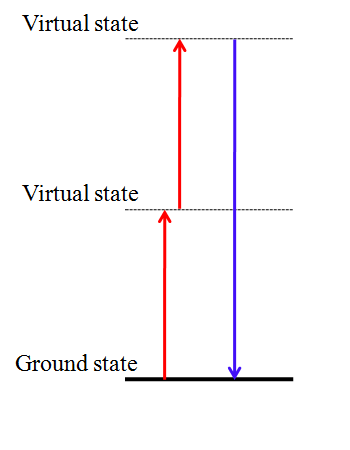
\includegraphics[width=0.3\textwidth]{media/Energy_level_scheme_of_SHG.png}
    \caption{Energy level scheme of SHG process. Taken from \cite{energy_level_scheme}.}
    \label{fig:energy_scheme}
\end{figure}


\section{Procedure}
\label{sec:procedure}

\subsection{Aligning the mirrors}
\label{sec:Aligning the mirrors}
The first step is to align every optical element, where we will start with the mirrors which will
later create the cavity.

For proper alignment of the optical elements, an optical axis should be defined. We did that with a
laser on a rail, the setting of which has to be constant throughout the experiment. The laser has to
be levelled with the rail, which has been achieved with a target on the opposite end of the rail.

The mirrors can be aligned by fixing them on the rail such that the reflect the laser beam back to
the source, as it is shown in \autoref{fig:aligning}. The mirror can then be aligned with its adjustments screws.
With curved mirrors, it is important to use a proper distance to the laser source. The reflection is
the most focused when the distance is the focal distance of the mirror, though this can be to small
to get an exact aligning. We managed to get meaningful results with approx. $\SI{30}{cm}$ of
distance for the alignment.

\begin{figure}
  \centering
  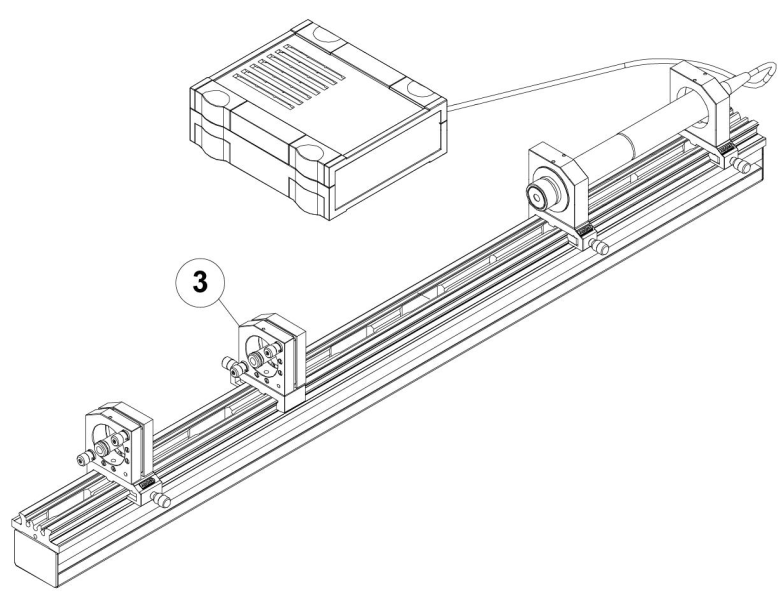
\includegraphics[width=0.45\textwidth]{media/aligning mirrors.png}
  \caption{Setup to align the mirrors. Item 3 corresponds to the mirror that can be adjusted in this
  position \cite{elas_manual}.}
  \label{fig:aligning}
\end{figure}

\subsection{Aligning the He-Ne tube}
\label{sec:Aligning the He-Ne tube}
The next step is to align the He-Ne tube, which can be done by removing the mirrors from the first
step. Than the laser and the target will be used to create a round beam shape. Here all four screws
should be used to achieve the highest range of motion.

\subsection{Creating the optical cavity}
\label{sec:Creating the optical cavity}
The last step is to position the mirrors pointing at each other with the He-Ne tube in between. Then
the reference laser can be turned off and power source of the Helium-Neon tube can be turned on.
Ideally, you get the laser oscillation right away. Practically, this is about as likely as getting an
A+ at KAIST. You can try to
shake around one mirror at a cavity length of $\SI{70}{cm}$ until you can fix it in a position where
you have a stable laser.

\begin{figure}
  \centering
  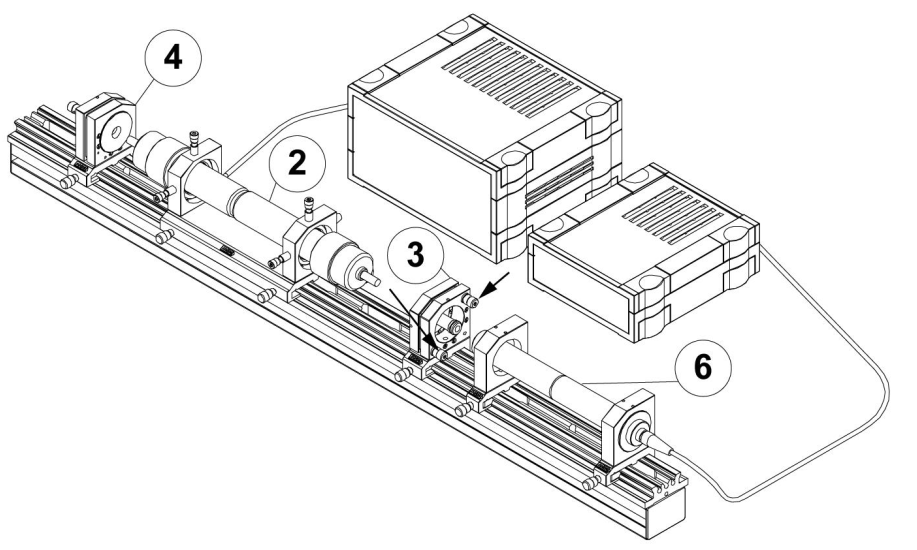
\includegraphics[width=0.45\textwidth]{media/setup.png}
  \caption{Final setup with the He-Ne tube (item 2) in the optical cavity (item 3,4). The reference laser (item 6)
  should be turned off and the He-Ne tube can be supplied with power \cite{elas_manual}.}
  \label{fig:setup}
\end{figure}

\section{Results}
\label{sec:results}

\subsection{Measurements taken by our group}

\begin{figure*}
  \centering
  \includegraphics{build/photocurrent_incorrect.pdf}
  \caption{Photo current for varying external voltages between sample and collector. Measurements taken by our own group. Note the linear relation between current and voltage for $U<0$.}
  \label{fig:photocurrent_own}
\end{figure*}

\section{Discussion}
\label{sec:discussion}
The ratio between the frequency peaks mentioned in \autoref{eqn:ratio} has a deviation of $0.2\%$
from a perfect frequency doubling.

Eventhough the result is close to the theoretical expectation, there have been many sources of
error which can lead to bad results. A perfect SHG has only be achieved after careful setup and
fine-tuning of the optical elements; small deviations can destroy the result altogether.

Apart from that, the rail and good quality of the elements made the procedure as stable as it was
for us.


\section{Conclusion}
\label{sec:conclusion}
This work found the speed of light in air and synthetic resin as
\begin{align}
  c_\text{Air} &= (2.97 \pm 0.04) 10^8 \, \si{ms^{-1}} \\
  c_\text{resin} &= (1.9 \pm 0.1) \cdot 10^8 \, \si{ms^{-1}},
\end{align}
the overall deviation from the known values taken from literature and experimental manual are less
or equal to $1.6\%$. The literature values lie within the boundries of uncertainty and for the
largest uncertainties the sources have been identiefied to be a low-quality probe and problems in
the experimental setup.



\appendix

\section{Letter encoding}
\label{sec:letter-encoding}
The letters get encoded by converting their index in a binary representation. To encode 26 letters,
the number of bits $n$ has to be so larger, such that $2^n \geq 26$, the smallest $n$ turns out to
be $5$. The whole scheme is shown in \autoref{tab:letter-encoding}, leaving only $6$ possible bits
empty.

\begin{table}
  \centering
  \caption{Binary representation of the alphabet, taken from \cite{thor_manual}.}
  \label{tab:letter-encoding}
  \sisetup{table-format=2.1}
  \begin{tabular}{c | c c c c c}
    A & 0 & 0 & 0 & 0 & 0 \\
    B & 0 & 0 & 0 & 0 & 1 \\
    C & 0 & 0 & 0 & 1 & 0 \\
    D & 0 & 0 & 0 & 1 & 1 \\
    E & 0 & 0 & 1 & 0 & 0 \\
    F & 0 & 0 & 1 & 0 & 1 \\
    G & 0 & 0 & 1 & 1 & 0 \\
    H & 0 & 0 & 1 & 1 & 1 \\
    I & 0 & 1 & 0 & 0 & 0 \\
    J & 0 & 1 & 0 & 0 & 1 \\
    K & 0 & 1 & 0 & 1 & 0 \\
    L & 0 & 1 & 0 & 1 & 1 \\
    M & 0 & 1 & 1 & 0 & 0 \\
    N & 0 & 1 & 1 & 0 & 1 \\
    O & 0 & 1 & 1 & 1 & 0 \\
    P & 0 & 1 & 1 & 1 & 1 \\
    Q & 1 & 0 & 0 & 0 & 0 \\
    R & 1 & 0 & 0 & 0 & 1 \\
    S & 1 & 0 & 0 & 1 & 0 \\
    T & 1 & 0 & 0 & 1 & 1 \\
    U & 1 & 0 & 1 & 0 & 0 \\
    V & 1 & 0 & 1 & 0 & 1 \\
    W & 1 & 0 & 1 & 1 & 0 \\
    X & 1 & 0 & 1 & 1 & 1 \\
    Y & 1 & 1 & 0 & 0 & 0 \\
    Z & 1 & 1 & 0 & 0 & 1 \\
  \end{tabular}
\end{table}



% The \nocite command causes all entries in a bibliography to be printed out
% whether or not they are actually referenced in the text. This is appropriate
% for the sample file to show the different styles of references, but authors
% most likely will not want to use it.
\nocite{*}

%\bibliography{apssamp}% Produces the bibliography via BibTeX.
\bibliography{lit}% Produces the bibliography via BibTeX.

\end{document}
%
% ****** End of file apssamp.tex ******
